\documentclass[a4paper,11pt,twoside]{article}
\usepackage[utf8]{inputenc}	% Text coding
\usepackage[T1]{fontenc}
\usepackage{lmodern}
\usepackage[czech]{babel}
\usepackage{epsfig}
\usepackage{amsfonts,amsmath,amssymb}
\usepackage{graphicx}
\usepackage[unicode]{hyperref}
\usepackage{indentfirst}
\usepackage{fancyhdr}
\usepackage{xifthen}
\usepackage{amsthm,thmtools}
\usepackage{bold-extra}
\usepackage[dvipsnames]{xcolor}
\usepackage[subrefformat=simple,labelformat=simple]{subcaption} % Instead of subfigure
\usepackage{listings}
\usepackage{comment}
\usepackage{titlesec}
\usepackage{underscore}
\usepackage{makecell}       % Šířky čar v tabulkách
\usepackage{wrapfig}

% Page size
\addtolength{\topmargin}{-1.5cm} %\addtolength{\textheight}{-10cm}
\addtolength{\textwidth}{4cm} \addtolength{\textheight}{4cm} % Width and height of the text
\addtolength{\voffset}{-0.5cm} % Top margin
\addtolength{\hoffset}{-2cm}
\setlength{\headheight}{15pt}

\DeclareMathOperator{\e}{e}

\def\vector#1{\boldsymbol{#1}}								% Vector
\renewcommand{\d}{\mathrm{d}}
\newcommand{\derivative}[3][]{\ifthenelse{\isempty{#1}}	    % Normal derivative
	{\frac{\d{#2}}{\d{#3}}}
	{\frac{\d^{#1}{#2}}{\d{#3}^{#1}}}
}
\newcommand{\im}{\mathrm{i}}

\def\makematrix#1{\begin{pmatrix}#1\end{pmatrix}}       % Matrix
\def\abs#1{\left|#1\right|}
\def\probability#1{\mathrm{Pr}\left[#1\right]}
\def\expectation#1{\mathrm{E}\left[#1\right]}
\def\dispersion#1{\sigma_{#1}^{2}}

\def\code#1{\textnormal{\texttt{#1}}}
\def\file#1{\textnormal{\textbf{\texttt{#1}}}}
\def\ghfile#1#2{\textnormal{\textbf{\texttt{\href{https://github.com/PavelStransky/PCInPhysics2021/blob/main/#1#2}{#2}}}}}

\def\abbreviation#1{\textnormal{\textsc{#1}}}

\begin{document}

\section*{Domácí úkol na 27.4.2023}
\subsection*{Rozdělení náhodných čísel}
Pro úspěšné vyřešení úkolu stačí správně naprogramovat jednu ze dvou úloh této sekce.
    \subsubsection*{1. Gaussovské rozdělení}
        Nagenerujte čísla vybraná z Gaussovského normálního rozdělení (se střední hodnotou $\mu=0$ a rozptylem $\sigma^{2}=1$) dvěma metodami: a) pomocí metody hit-and-miss a b) pomocí centrální limitní věty.
        Nakreslete a porovnejte histogramy.

    \subsubsection*{2. Cauchyho rozdělení}
        Vytvořte dva generátory čísel z rozdělení daného distribuční funkcí
        \begin{equation*}
            F(x)=\frac{1}{2}\left(1+\frac{2}{\pi}\arctan{x}\right).
        \end{equation*}
        V prvním generátoru využijte přímo distribuční funkci, pro druhý odvoďte hustotu pravděpodobnosti a použijte hit-and-miss metodu.
        Nakreslete a porovnejte histogramy.

\subsection*{Monte Carlo}
Pro úspěšné vyřešení úkolu stačí správně naprogramovat dvě ze tří úloh této sekce.
\subsubsection*{3. Narozeninový problém}
    Uvažujte skupinu $n$ lidí. 
    Jaká je pravděpodobnost, že dvě osoby ve skupině budou mít narozeniny ve stejný den? 
    Úlohu vyřešte metodou Monte Carlo: 
    Pokud nagenerujete náhodně $N_\text{celkem}$-krát narozeniny $n$ lidí a označíte $N_{\text{zásah}}$ případy, kdy alespoň dvoje narozeniny padnou na stejný den, 
    bude podle zákona velkých čísel hledaná pravděpodobnost rovna
    \begin{equation*}
        p\approx\frac{N_{\text{zásah}}}{N_{\text{celkem}}}
    \end{equation*}
    Naprogramujte tuto úlohu a určete,

    \begin{itemize}
        \item jaká pravděpodobnost vychází pro skupinu 20 lidí a
        \item jakou nejmenší skupinu potřebujete, aby byla pravděpodobnost alespoň 90\%?
    \end{itemize}

\subsubsection*{4. Objem $d$-rozměrné koule}
    Vytvořte program, který spočítá metodou Monte Carlo objem $d$-rozměrné jednotkové koule.
    Pro jakou dimenzi $d$ bude tento objem největší číslo?

\subsubsection*{5. Gaussovka na srdci}
    \begin{wrapfigure}{r}{5cm}
        \centering
        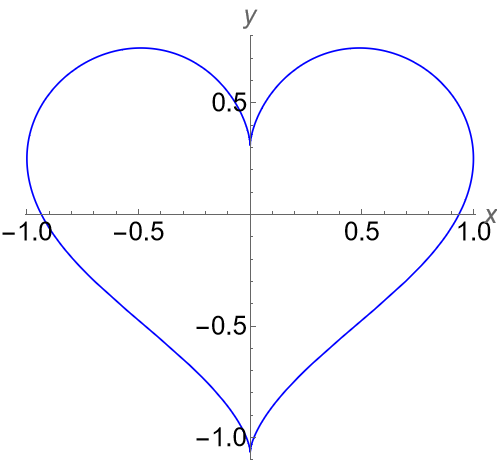
\includegraphics[width=\linewidth]{heart.png}
    \end{wrapfigure}
    Metodou Monte Carlo vypočítejte integrál dvourozměrné Gaussovské funkce
    \begin{equation*}
        I=\int_{\heartsuit}\frac{1}{2\pi}\e^{-\frac{1}{2}\left(x^{2}+y^{2}\right)}\d x\,\d y
    \end{equation*}
    na oblasti ohraničené parametricky zadanou křivkou (obrázek):
    \begin{align*}
        \heartsuit: 
            x&=\sin^{3}{\phi},\\
            y&=\frac{1}{16}\left(13\cos{\phi}-5\cos{2\phi}-2\cos{3\phi}-\cos{4\phi}\right),\\
            \phi&\in\langle0;2\pi).
    \end{align*}
\end{document}



\end{document}